\documentclass[hyper, linkcolor=blue]{mythesis}

\usepackage{mystyle}
\usepackage[colorinlistoftodos]{todonotes}
\graphicspath{{./figures/}}
\makeatother

\title{Discovery of the Higgs boson in the \WW decay channel using the ATLAS detector at the Large Hadron Collider}
\author{David Christopher Hall}

%\includeonly{}
\begin{document}
%TC:ignore
\begin{frontmatter}
  %!TEX root = ../thesis.tex

%% Title
\titlepage[\vspace{12pt}St Catherine's College, University of Oxford]{
\vspace{-140pt}
\begin{figure}[ht]
	\begin{minipage}[b]{0.35\linewidth}
		\centering
		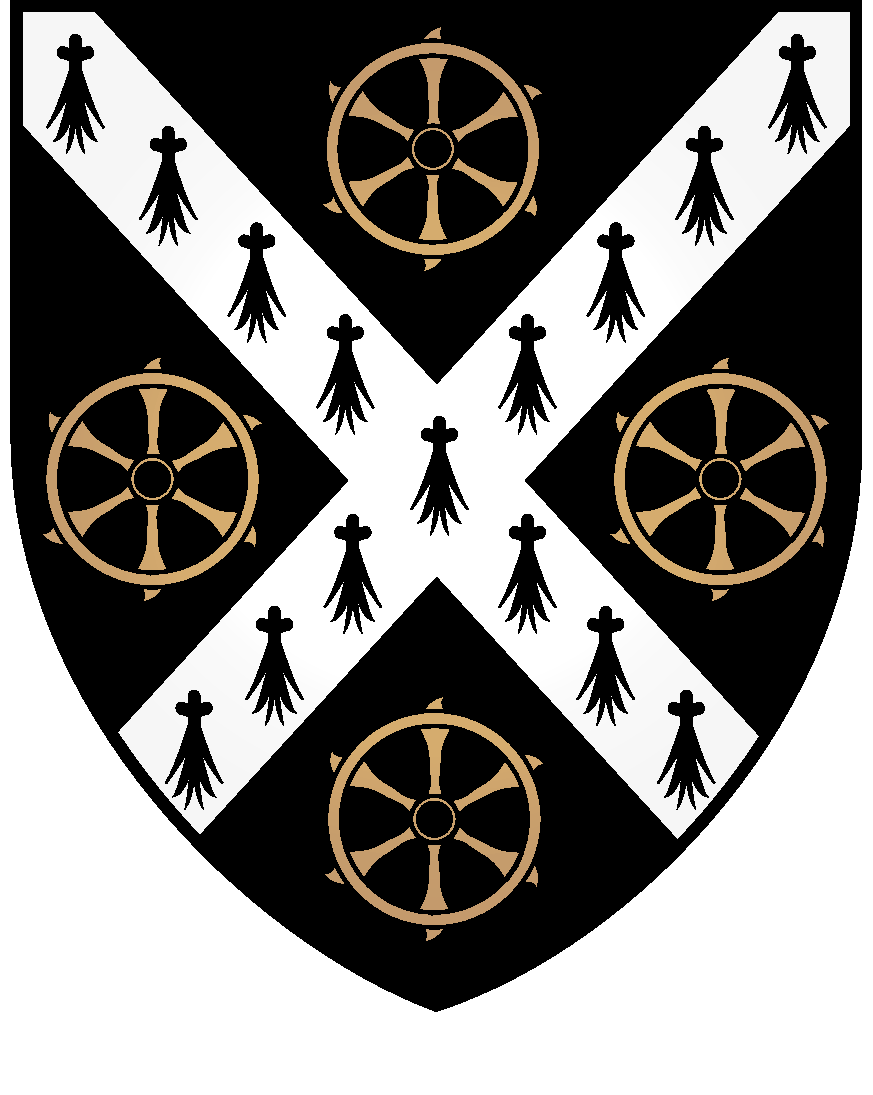
\includegraphics[height=4.5cm]{tex/catz-arms.pdf}
	\end{minipage}
	\hspace{0.5cm}
	\begin{minipage}[b]{0.35\linewidth}
		\centering
		
\includegraphics[height=4.5cm]{tex/ox-logo.pdf}
	\end{minipage}
\end{figure}
\vspace{20pt}
Submitted in partial fulfilment of the requirements\\ 
for the degree of Doctor of Philosophy\\
Trinity 2014}

%% Abstract
\begin{abstract}%[\smaller \thetitle\\ \vspace*{1cm} \smaller {\theauthor}]
  %\thispagestyle{empty}
  %!TEX root = ../thesis.tex

In the Standard Model of particle physics, the non-zero masses of the \PW and \PZ bosons and 
the fermions are generated through interactions with the Higgs field, excitations of which 
correspond to Higgs bosons. Thus, the experimental discovery of the Higgs boson is of prime 
importance to physics, and would confirm our understanding of fundamental mass generation.

This thesis describes a search for the \ggHWWlvlv process of Higgs boson production and decay.
It uses the LHC Run~I dataset of \pp collisions recorded by the ATLAS detector, which 
corresponds to an integrated luminosity of \unit{4.5}{\invfb} at \unit{$\sqrt{s} = 7$}{\TeV} 
and \unit{20.3}{\invfb} at \unit{$\sqrt{s} = 8$}{\TeV}. An excess of events is observed, 
consistent with Higgs boson production, with a significance of 5.3 standard deviations at 
\unit{$\mH = 125$}{\GeV}. The measured signal strength is $1.14^{+0.28}_{-0.24}$ at 
\unit{$\mH = 125$}{\GeV}. A cross section measurement of \WW production, a major background 
to this search, is also presented using the \unit{$\sqrt{s} = 7$}{\TeV} dataset only.

\end{abstract}

%% Acknowledgements
\begin{acknowledgements}
  %!TEX root = ../thesis.tex

Thank you, thank you

\end{acknowledgements}

%% Preface
\begin{preface}
  %!TEX root = ../thesis.tex

As a DPhil research topic, the \HWW analysis has proven to be a baptism of fire. It is the 
most complicated of the three ``discovery channels'',\footnote{
	The \HepProcess{\Pphoton\Pphoton}, \ZZ and \WW decay channels quickly gave sensitivity 
	to the Higgs boson ultimately discovered.
}
as it involves a variety of physics objects and requires a good understanding of many 
difficult backgrounds. As such, the analysis took huge effort from a large number of 
individuals. My role focussed on theoretical aspects of the signal and background 
modelling, and these parts shall be emphasised. I contributed to multiple iterations of 
the analysis \cite{ATLAS-discovery,HWW-HCP,HWW-Moriond}, though the version presented here 
is unpublished at the time of writing. I also co-authored the third Yellow Report 
produced by the LHC Higgs Cross Section Working Group \cite{YR3}.

When I began the degree in October 2010, there was no direct evidence for a Higgs boson. 
This thesis is written from a personal perspective and motivates a low mass search by 
electroweak fits, when in fact this aspect was motivated later by observations of a 
resonance in the \HepProcess{\Pphoton\Pphoton} and \ZZ channels.\footnote{
	Dedicated high mass searches for \HWW have also been performed \cite{HWW-highmass}.
}
Also, an advanced search strategy is described, though the discovery of \HWW was actually 
a gradual process with multiple iterations of blinding, optimising and unblinding the 
analysis. As more data were recorded and the analysis was enhanced, the results improved.

Early on, I gained relevant insight through \WW cross section measurements 
\cite{WW-1ifb,WW-HCP,WW-7TeV}. My main contribution was a jet veto correction factor 
applied to the \WW signal, which reduces the dominant uncertainty in the analysis. This 
measurement shall be described when considering the \WW background to the \HWW search.

To qualify for authorship within the ATLAS collaboration, I performed Run Control shifts. 
I also worked within the Versatile Link project \cite{VersatileLink} to investigate 
radiation hardened optical components for future particle physics experiments. As this 
research does not easily relate to the Higgs boson, it is excluded from this thesis. 
However, I have published articles on the radiation tolerance of optical fibres 
\cite{VersatileLinkFibres} and their connectors \cite{VersatileLinkConnectors}.

\end{preface}

%% ToC
\setcounter{tocdepth}{1}
\tableofcontents

\end{frontmatter}
%TC:endignore

\begin{mainmatter}
  \listoftodos
  %!TEX root = ../thesis.tex

The Standard Model of particle physics describes the behaviour of sub-atomic particles. 
Since its formulation in the 1970s, it has experienced unparalleled success in modelling a 
wide range of phenomena; no experimental result within the remit of the Standard Model is 
currently considered to significantly contradict its validity.\footnote{
	Observation of neutrino oscillations required neutrino masses to be manually added to 
	the Standard Model. It is widely believed that their relatively small masses will be 
	explained by new physics.
}
However, there are a number of physical phenomena that the Standard Model is unable to 
describe: gravitational attraction between massive objects, the observed asymmetry between 
matter and antimatter in the Universe, and astronomical evidence for dark matter and the 
cosmological constant.

A crucial aspect of the Standard Model is how non-zero masses are imparted to fundamental 
particles. These are forbidden by underlying symmetries of the theory, though remain an 
experimental fact; for example, atoms could not form if the electron did not possess mass.
This is achieved via interactions with a ubiquitous Higgs field, excitations of which 
correspond to Higgs bosons. As the only undiscovered particle of the Standard Model, the 
discovery of the Higgs boson is of utmost importance to particle physics: it would complete 
our knowledge of the Standard Model, and in particular confirm the mechanism of mass 
generation. As such, it was a primary goal of the LHC physics program, which began in 2010.

This thesis describes the search, discovery and measurement of the Higgs boson using 
proton-proton collision data recorded by the ATLAS experiment at CERN. This is accomplished 
by searching for collisions where a Higgs boson is produced and subsequently decays to two 
\PW bosons, each of which decay to an electron or muon and a neutrino (\ie \HWWlvlv). This 
search suffers from large experimental backgrounds, such as continuum \WW production, which 
must be accurately modelled to yield sensitivity to the Higgs boson.

First, the theoretical motivation for the Higgs boson is presented in 
\Chapter~\ref{chap:motivation}. Then, \Chapter~\ref{chap:tools} outlines some important 
concepts related to making precise predictions within the Standard Model, which shall be 
referred to throughout the thesis. The experimental setup of the LHC and the ATLAS detector 
are described in \Chapter~\ref{chap:experiment}.

Focus then moves to the data analysis itself. \Chapter~\ref{chap:selection} offers an 
overview of the entire \HWW analysis, detailing the selection of Higgs boson signal events 
and the rejection of backgrounds. Following this, signal modelling is described in 
\Chapter~\ref{chap:signal}, \WW background modelling is described in \Chapter~\ref{chap:ww} 
(including a dedicated cross section measurement), and the modelling of other backgrounds is 
described in \Chapter~\ref{chap:backgrounds}. The experimental results are presented and 
discussed in \Chapter~\ref{chap:results}. Finally, in \Chapter~\ref{chap:conclusions}, we 
draw conclusions from the results of this analysis and of others conducted simultaneously at 
the LHC, and consider the outlook of Higgs physics.

  \part{Theoretical and Experimental Background}
    %!TEX root = ../thesis.tex

\chapter{The Standard Model of Particle Physics}
\section{Section}
\subsection{Sub-section}
\cite{Stewart-Tackmann:2012}

    \include{tex/montecarlo}
    \include{tex/detector}

  \part{Standard Model \WW cross section measurement}

  \part{\HWW discovery}
    \include{tex/ww}
    \include{tex/signal}
    \include{tex/wgammastar}

\end{mainmatter}

\begin{appendices}

\end{appendices}

\begin{backmatter}
  \bibliographystyle{h-physrev}
  %\bibliographystyle{plain}
  \bibliography{theory, mc, experiment}
  \listoffigures
  \listoftables
\end{backmatter}

\end{document}
